% Options for packages loaded elsewhere
% Options for packages loaded elsewhere
\PassOptionsToPackage{unicode}{hyperref}
\PassOptionsToPackage{hyphens}{url}
\PassOptionsToPackage{dvipsnames,svgnames,x11names}{xcolor}
%
\documentclass[
  letterpaper,
]{article}
\usepackage{xcolor}
\usepackage[margin=1in]{geometry}
\usepackage{amsmath,amssymb}
\setcounter{secnumdepth}{5}
\usepackage{iftex}
\ifPDFTeX
  \usepackage[T1]{fontenc}
  \usepackage[utf8]{inputenc}
  \usepackage{textcomp} % provide euro and other symbols
\else % if luatex or xetex
  \usepackage{unicode-math} % this also loads fontspec
  \defaultfontfeatures{Scale=MatchLowercase}
  \defaultfontfeatures[\rmfamily]{Ligatures=TeX,Scale=1}
\fi
\usepackage{lmodern}
\ifPDFTeX\else
  % xetex/luatex font selection
\fi
% Use upquote if available, for straight quotes in verbatim environments
\IfFileExists{upquote.sty}{\usepackage{upquote}}{}
\IfFileExists{microtype.sty}{% use microtype if available
  \usepackage[]{microtype}
  \UseMicrotypeSet[protrusion]{basicmath} % disable protrusion for tt fonts
}{}
\makeatletter
\@ifundefined{KOMAClassName}{% if non-KOMA class
  \IfFileExists{parskip.sty}{%
    \usepackage{parskip}
  }{% else
    \setlength{\parindent}{0pt}
    \setlength{\parskip}{6pt plus 2pt minus 1pt}}
}{% if KOMA class
  \KOMAoptions{parskip=half}}
\makeatother
% Make \paragraph and \subparagraph free-standing
\makeatletter
\ifx\paragraph\undefined\else
  \let\oldparagraph\paragraph
  \renewcommand{\paragraph}{
    \@ifstar
      \xxxParagraphStar
      \xxxParagraphNoStar
  }
  \newcommand{\xxxParagraphStar}[1]{\oldparagraph*{#1}\mbox{}}
  \newcommand{\xxxParagraphNoStar}[1]{\oldparagraph{#1}\mbox{}}
\fi
\ifx\subparagraph\undefined\else
  \let\oldsubparagraph\subparagraph
  \renewcommand{\subparagraph}{
    \@ifstar
      \xxxSubParagraphStar
      \xxxSubParagraphNoStar
  }
  \newcommand{\xxxSubParagraphStar}[1]{\oldsubparagraph*{#1}\mbox{}}
  \newcommand{\xxxSubParagraphNoStar}[1]{\oldsubparagraph{#1}\mbox{}}
\fi
\makeatother


\usepackage{longtable,booktabs,array}
\usepackage{calc} % for calculating minipage widths
% Correct order of tables after \paragraph or \subparagraph
\usepackage{etoolbox}
\makeatletter
\patchcmd\longtable{\par}{\if@noskipsec\mbox{}\fi\par}{}{}
\makeatother
% Allow footnotes in longtable head/foot
\IfFileExists{footnotehyper.sty}{\usepackage{footnotehyper}}{\usepackage{footnote}}
\makesavenoteenv{longtable}
\usepackage{graphicx}
\makeatletter
\newsavebox\pandoc@box
\newcommand*\pandocbounded[1]{% scales image to fit in text height/width
  \sbox\pandoc@box{#1}%
  \Gscale@div\@tempa{\textheight}{\dimexpr\ht\pandoc@box+\dp\pandoc@box\relax}%
  \Gscale@div\@tempb{\linewidth}{\wd\pandoc@box}%
  \ifdim\@tempb\p@<\@tempa\p@\let\@tempa\@tempb\fi% select the smaller of both
  \ifdim\@tempa\p@<\p@\scalebox{\@tempa}{\usebox\pandoc@box}%
  \else\usebox{\pandoc@box}%
  \fi%
}
% Set default figure placement to htbp
\def\fps@figure{htbp}
\makeatother





\setlength{\emergencystretch}{3em} % prevent overfull lines

\providecommand{\tightlist}{%
  \setlength{\itemsep}{0pt}\setlength{\parskip}{0pt}}



 


\usepackage{booktabs}
\usepackage{longtable}
\usepackage{float}
\usepackage{needspace}
\renewenvironment{abstract}{\par\bigskip\noindent\textbf{Abstract}\par\smallskip}{\par\bigskip}
\makeatletter
\@ifpackageloaded{caption}{}{\usepackage{caption}}
\AtBeginDocument{%
\ifdefined\contentsname
  \renewcommand*\contentsname{Table of contents}
\else
  \newcommand\contentsname{Table of contents}
\fi
\ifdefined\listfigurename
  \renewcommand*\listfigurename{List of Figures}
\else
  \newcommand\listfigurename{List of Figures}
\fi
\ifdefined\listtablename
  \renewcommand*\listtablename{List of Tables}
\else
  \newcommand\listtablename{List of Tables}
\fi
\ifdefined\figurename
  \renewcommand*\figurename{Figure}
\else
  \newcommand\figurename{Figure}
\fi
\ifdefined\tablename
  \renewcommand*\tablename{Table}
\else
  \newcommand\tablename{Table}
\fi
}
\@ifpackageloaded{float}{}{\usepackage{float}}
\floatstyle{ruled}
\@ifundefined{c@chapter}{\newfloat{codelisting}{h}{lop}}{\newfloat{codelisting}{h}{lop}[chapter]}
\floatname{codelisting}{Listing}
\newcommand*\listoflistings{\listof{codelisting}{List of Listings}}
\makeatother
\makeatletter
\makeatother
\makeatletter
\@ifpackageloaded{caption}{}{\usepackage{caption}}
\@ifpackageloaded{subcaption}{}{\usepackage{subcaption}}
\makeatother
\usepackage{bookmark}
\IfFileExists{xurl.sty}{\usepackage{xurl}}{} % add URL line breaks if available
\urlstyle{same}
\hypersetup{
  pdftitle={Administrative Throughput and Disaster Recovery Timeliness: An Exploratory Cross-Sectional SEM Assessment of CDBG-DR Fund Management},
  pdfauthor={Kai-Fa Lu; Jesse Andrews; Ali Nejat},
  colorlinks=true,
  linkcolor={blue},
  filecolor={Maroon},
  citecolor={Blue},
  urlcolor={Blue},
  pdfcreator={LaTeX via pandoc}}


\title{Administrative Throughput and Disaster Recovery Timeliness: An
Exploratory Cross-Sectional SEM Assessment of CDBG-DR Fund Management}
\author{Kai-Fa Lu \and Jesse Andrews \and Ali Nejat}
\date{}
\begin{document}
\maketitle

\renewcommand*\contentsname{Table of contents}
{
\hypersetup{linkcolor=}
\setcounter{tocdepth}{3}
\tableofcontents
}

\section*{Abstract}\label{abstract}
\addcontentsline{toc}{section}{Abstract}

This archived manuscript evaluates whether grantee-level financial-flow
indicators from HUD's Disaster Recovery Grant Reporting (DRGR) Quarterly
Performance Reports (QPRs) can support a defensible cross-sectional
structural equation model (SEM) of administrative throughput in the
Community Development Block Grant-Disaster Recovery (CDBG-DR) program.
The reproducible archive supports descriptive comparisons across 156
grantee-disaster observations, 78 unique grantees, and 18 disaster
contexts linked to disaster cohorts from 2003 through 2023; however, the
SEM evidence is substantially weaker than the latest Word manuscript
claims. Across the archived model-comparison files, no single
specification is preferred on all fit criteria. The legacy
three-indicator state replication can reproduce a large positive path
from the latent throughput factor to recovery outcome, but that result
depends on right-censored duration and the use of timeliness as the
inverse of the same duration measure. Simpler non-circular models with
complete-case samples of 40 to 41 grantees and subset samples of 23
states or 17 local governments do not yield stable or statistically
persuasive structural paths. Accordingly, this redraft treats the SEM
results as exploratory associations rather than confirmatory evidence
that administrative throughput determines recovery outcomes. The main
contribution of the archive is therefore methodological: it documents
how grantee-level aggregation, maturity censoring, and indicator choice
shape the feasibility of SEM in this setting and why a longitudinal or
event-history redesign is needed for stronger causal or policy claims.

\section{Introduction}\label{introduction}

Administrative capacity is central to long-run disaster recovery, but it
is hard to observe directly. In the CDBG-DR program, state agencies,
counties, cities, and territories receive flexible federal funds for
recovery and mitigation, yet they move those funds through obligation,
disbursement, and expenditure at very different rates. The practical
question is whether those differences reflect an underlying throughput
pattern that can be summarized consistently across jurisdictions.

The archived Kaifa manuscript attempted to answer that question with a
cross-sectional SEM built from quarterly QPR data. That ambition remains
worth pursuing, but the current repository no longer supports the
stronger claims made in the latest Word draft. The active project audit
found three core problems. First, the quantitative backbone is
internally inconsistent: the later Word draft, the archived Quarto
source, and the reproducible diagnostic tables do not tell the same
model-selection story. Second, the main positive SEM result depends on a
legacy design that censors duration at the current observation window
and then uses timeliness as the inverse of that same duration, creating
mathematical coupling between the latent constructs. Third, the
available complete-case SEM samples are too small for confident
state-versus-local comparisons.

This redraft therefore narrows the manuscript to a more defensible goal:
an exploratory assessment of whether grantee-level financial throughput
indicators can sustain a cross-sectional SEM at all. The paper makes
four claims.

\begin{enumerate}
\def\labelenumi{\arabic{enumi}.}
\tightlist
\item
  The descriptive QPR ratios show meaningful cross-grantee variation in
  the movement of funds from obligation to disbursement.
\item
  The archived SEM specifications do not produce a single robust,
  confirmatory measurement model.
\item
  The strong positive state-level path reported in the later Word draft
  is reproducible only under a legacy specification with known design
  flaws.
\item
  Any future manuscript that wants to reintroduce staffing, social
  vulnerability, or geography-sensitive covariates needs a separate
  reproducibility rebuild before those variables can be interpreted with
  confidence.
\end{enumerate}

The current manuscript is therefore a salvage and transparency exercise,
not a submission-ready empirical paper.

\section{Background}\label{background}

\subsection{Recovery Governance and Implementation
Capacity}\label{recovery-governance-and-implementation-capacity}

Disaster recovery depends on the capacity of implementing organizations
to translate federal allocations into completed programs. In the
intergovernmental system that governs CDBG-DR, state and local grantees
must navigate federal reporting requirements, coordinate across
agencies, and manage administrative processes that can span a decade or
more. Public administration scholarship emphasizes that this
implementation capacity is multidimensional: it involves organizational
resources, administrative routines, institutional coordination, and the
ability to absorb and deploy funds under pressure (Wu, Ramesh, and
Howlett 2015). Administrative burden research further highlights that
procedural demands fall unevenly on organizations with different
staffing levels and institutional arrangements, creating systematic
variation in throughput that is difficult to capture with any single
measure (Gerber and Robinson 2022).

\subsection{Measurement Challenge}\label{measurement-challenge}

SEM is attractive in this context because it can represent throughput as
a latent factor rather than a single ratio. That advantage comes with a
cost: the measurement model must be empirically defensible. A latent
factor is only as credible as its indicators, fit diagnostics, and
identification logic. Small samples, overlapping indicators, and
unstable subset estimates can make an elegant SEM narrative look
stronger than the underlying evidence warrants. The Kaifa archive is
useful because it documents both the promising and problematic paths:
the legacy replication that produced a large positive coefficient and
several alternative non-circular specifications that do not support the
same conclusion.

\section{Data And Cross-Sectional
Design}\label{data-and-cross-sectional-design}

The reproducible archive uses the project-standardized QPR pipeline and
its derived grantee-disaster panel. The working parquet files show
quarterly QPR observations from September 30, 2002 through June 30,
2025. To keep the manuscript aligned with the disaster cohorts actually
discussed in the archived SEM figures and tables, the redraft refers to
disaster events from 2003 through 2023. The panel used for SEM
sensitivity work contains 156 grantee-disaster pairs, 78 unique
grantees, and 18 disaster types.

Terminology is fixed as follows throughout the manuscript:

\begin{itemize}
\tightlist
\item
  \texttt{grantee}: the state or local governmental recipient
  responsible for a CDBG-DR allocation.
\item
  \texttt{grant} or \texttt{disaster\ allocation}: the disaster-specific
  CDBG-DR award associated with a grantee-disaster pair.
\item
  \texttt{activity}: an underlying DRGR/QPR record inside a
  grantee-disaster quarter.
\item
  \texttt{grantee-disaster\ pair}: the main unit of analysis before
  cross-sectional aggregation.
\end{itemize}

The main cross-sectional SEM collapses the grantee-disaster panel to one
mean profile per grantee. That choice assumes a jurisdiction's
administrative style is stable enough across disasters to summarize as a
cross-sectional trait. The manuscript no longer treats that assumption
as innocuous. It is a strong modeling decision that trades away
within-grantee variation, cohort differences, and institutional change
over time. State and local results are therefore presented only as
subset sensitivity checks, not as formal moderation analyses. The pooled
model assumes approximate measurement equivalence across institutional
types, which has not been formally tested. State agencies typically
administer CDBG-DR through centralized offices with dedicated
disaster-recovery staff, while local governments often manage grants
through general-purpose community development departments with competing
priorities. This institutional heterogeneity means that identical
throughput ratios may reflect different administrative realities.
Clustered standard errors, which would account for within-type
correlation, would likely widen confidence intervals beyond those
reported here.

The redraft also distinguishes clearly between the current Quarto
archive and the later April 7, 2026 Word draft. The Word draft refers to
BLS QCEW staffing measures, CDC/ATSDR Social Vulnerability Index (SVI)
data, and city-to-county geography matching. Those extensions are not
fully reconstructed in the current reproducible Quarto archive and are
therefore not treated as active empirical inputs in the results reported
here. Their provenance boundary is documented in Appendix A.

\section{Measures}\label{measures}

\subsection{Throughput Indicators}\label{throughput-indicators}

The archive contains several candidate indicators for a latent
throughput factor:

\begin{itemize}
\tightlist
\item
  \texttt{Ratio\_disbursed\_to\_obligated}: the share of obligated funds
  that have moved into disbursement.
\item
  \texttt{Ratio\_expended\_to\_disbursed}: the share of disbursed funds
  that have been expended.
\item
  \texttt{Timeliness\_censored}: the inverse of a right-censored
  duration variable used only in the legacy replication model.
\end{itemize}

The first two indicators capture financial throughput. The third is a
legacy indicator retained only to document how the original positive
result was obtained; it is not used as a preferred measure because it is
mechanically linked to the duration outcome.

These indicators are indirect throughput proxies, not direct measures of
organizational capacity. The fund-flow ratios capture how quickly money
moves through the federal pipeline but do not distinguish whether
throughput reflects grantee administrative effort, HUD processing speed,
or program design constraints. The manuscript therefore refers to the
latent factor as a throughput summary rather than a validated capacity
measure.

A further specification tension concerns whether the indicators are best
understood as reflective manifestations of a single latent trait or as
formative components that jointly constitute throughput. In a reflective
specification, each ratio is caused by an underlying administrative
dimension; in a formative specification, the indicators are determinants
of a composite. The SEMs reported here adopt a reflective specification
for estimation convenience, but this choice is not validated. The factor
loadings should be read as exploratory summaries of covariation, not as
evidence that a single latent trait generates the observed indicators.

\subsection{Recovery Outcome
Indicators}\label{recovery-outcome-indicators}

The archive also contains several outcome-side indicators:

\begin{itemize}
\tightlist
\item
  \texttt{Duration\_log}: log-transformed completion time for
  grantee-disaster pairs that reach the completion threshold.
\item
  \texttt{Spending\_CV}: the coefficient of variation of quarterly
  expenditure flows.
\item
  \texttt{Duration\_censored}: a legacy duration that substitutes
  observed program age when completion is not reached.
\item
  \texttt{Ratio\_obligated\_funds\_fully\_expended}: the share of
  obligated funds fully expended by the end of the observation window.
\item
  \texttt{Quarter\_by\_quarter\_variance\_expended}: normalized
  quarter-to-quarter variability in expenditures.
\item
  \texttt{Time\_to\_50pct}: the normalized quarters needed to reach 50
  percent completion.
\end{itemize}

The manuscript treats the duration-based measures cautiously. Any
outcome defined at 95 percent completion is vulnerable to maturity bias
and right-censoring, especially for more recent disasters. That is why
the cross-sectional SEM is framed as exploratory and why the preferred
baseline specification avoids the direct timeliness-versus-duration
overlap used in the legacy replication.

\section{Audit-Informed Model
Comparison}\label{audit-informed-model-comparison}

The first priority in the revision plan was to reconcile the model
comparison narrative with the archived outputs. Table 1 reproduces the
specification comparison from the manuscript-specific robustness file in
the Quarto archive.

\begin{longtable}[]{@{}
  >{\raggedright\arraybackslash}p{(\linewidth - 14\tabcolsep) * \real{0.1000}}
  >{\raggedleft\arraybackslash}p{(\linewidth - 14\tabcolsep) * \real{0.1333}}
  >{\raggedleft\arraybackslash}p{(\linewidth - 14\tabcolsep) * \real{0.1333}}
  >{\raggedleft\arraybackslash}p{(\linewidth - 14\tabcolsep) * \real{0.1333}}
  >{\raggedleft\arraybackslash}p{(\linewidth - 14\tabcolsep) * \real{0.1333}}
  >{\raggedleft\arraybackslash}p{(\linewidth - 14\tabcolsep) * \real{0.1333}}
  >{\raggedleft\arraybackslash}p{(\linewidth - 14\tabcolsep) * \real{0.1333}}
  >{\raggedright\arraybackslash}p{(\linewidth - 14\tabcolsep) * \real{0.1000}}@{}}
\toprule\noalign{}
\begin{minipage}[b]{\linewidth}\raggedright
Model
\end{minipage} & \begin{minipage}[b]{\linewidth}\raggedleft
N
\end{minipage} & \begin{minipage}[b]{\linewidth}\raggedleft
CFI
\end{minipage} & \begin{minipage}[b]{\linewidth}\raggedleft
TLI
\end{minipage} & \begin{minipage}[b]{\linewidth}\raggedleft
RMSEA
\end{minipage} & \begin{minipage}[b]{\linewidth}\raggedleft
AIC
\end{minipage} & \begin{minipage}[b]{\linewidth}\raggedleft
BIC
\end{minipage} & \begin{minipage}[b]{\linewidth}\raggedright
Audit note
\end{minipage} \\
\midrule\noalign{}
\endhead
\bottomrule\noalign{}
\endlastfoot
\texttt{full} & 41 & 0.938 & 0.883 & 0.152 & 25.250 & 47.526 & Best
conventional CFI/TLI among archived models, but uses overlapping timing
indicators. \\
\texttt{reduced} & 41 & 0.498 & -0.256 & 0.572 & 19.253 & 38.102 &
Clearly poor fit. \\
\texttt{exp\_optimal\_v1} & 40 & 0.790 & -0.259 & 0.000 & 17.999 &
33.199 & Lowest AIC/BIC and non-circular baseline, but low incremental
fit. \\
\texttt{exp\_optimal\_v2} & 40 & 0.758 & 0.394 & 0.000 & 21.865 & 40.442
& No fit improvement over \texttt{exp\_optimal\_v1}. \\
\texttt{improved\_3x3} & 40 & 1.486 & 1.911 & 0.000 & 25.795 & 47.751 &
Apparent overfit with inadmissible CFI/TLI values in a very small
sample. \\
\texttt{improved\_3x3\_progress} & 40 & 0.238 & -0.430 & 0.396 & 23.150
& 45.105 & Poor fit and not interpretable. \\
\end{longtable}

Table 1 eliminates the contradiction that appeared in the Word
manuscript: the archive does not support a clean statement that one
model is best on all major indices. The \texttt{full} model has the
strongest conventional CFI/TLI among the archived specifications, but
its RMSEA is poor and its indicator set is conceptually compromised by
the timing overlap. The non-circular \texttt{exp\_optimal\_v1} model has
the lowest AIC and BIC, but its low CFI means it cannot be presented as
a well-fitting confirmatory solution. The \texttt{improved\_3x3} values
exceed the usual upper bound for CFI and TLI, which is another sign that
the sample is too small for confident interpretation.

The manuscript therefore adopts the following transparent rule. The
\texttt{exp\_optimal\_v1} model is treated as the least problematic
baseline because it avoids the timeliness-duration circularity. The
\texttt{full} 3x3 model is reported only as a legacy comparison that
helps explain how the original positive manuscript result was generated.
No specification is treated as a validated measurement model.

\section{Results}\label{results}

\subsection{Descriptive Throughput
Patterns}\label{descriptive-throughput-patterns}

The descriptive ratio figures remain the strongest part of the archive.
State-level average ratios show that once funds are disbursed they are
usually expended efficiently, whereas the main throughput bottleneck
occurs earlier in the pipeline between obligation and disbursement.

\begin{figure}[H]

{\centering \pandocbounded{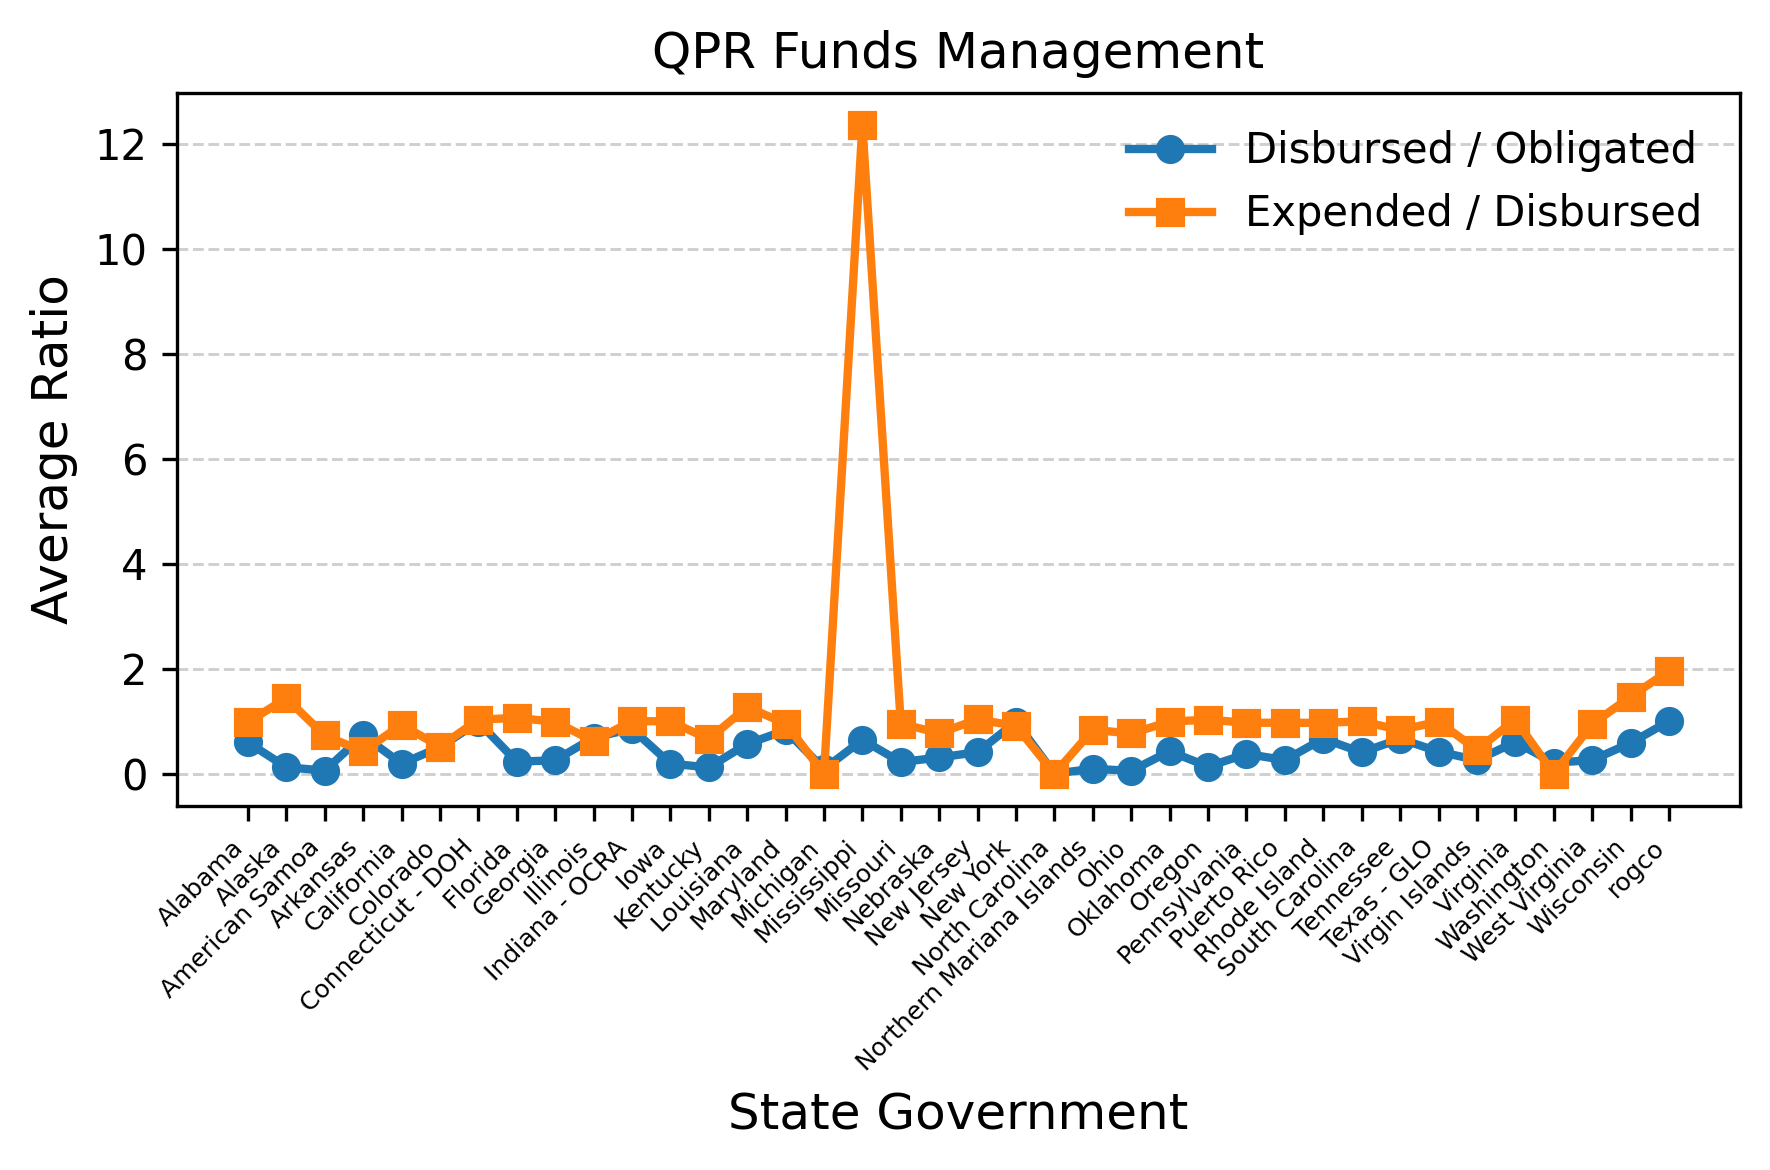
\includegraphics[keepaspectratio]{figures/fig_08_state_avg_ratios_2003_2023.png}}

}

\caption{Quarterly average state-level QPR ratios, showing greater
variation in the movement from obligation to disbursement than in the
movement from disbursement to expenditure across disaster cohorts from
2003 through 2023.}

\end{figure}%

Local governments display a similar pattern but with generally lower
disbursed-to-obligated ratios and more visible heterogeneity in a small
number of jurisdictions. The descriptive contrast is useful, but it
should not be overstated as direct evidence of a latent
state-versus-local throughput difference because the later SEM subset
samples are small and unstable.

\begin{figure}[H]

{\centering \pandocbounded{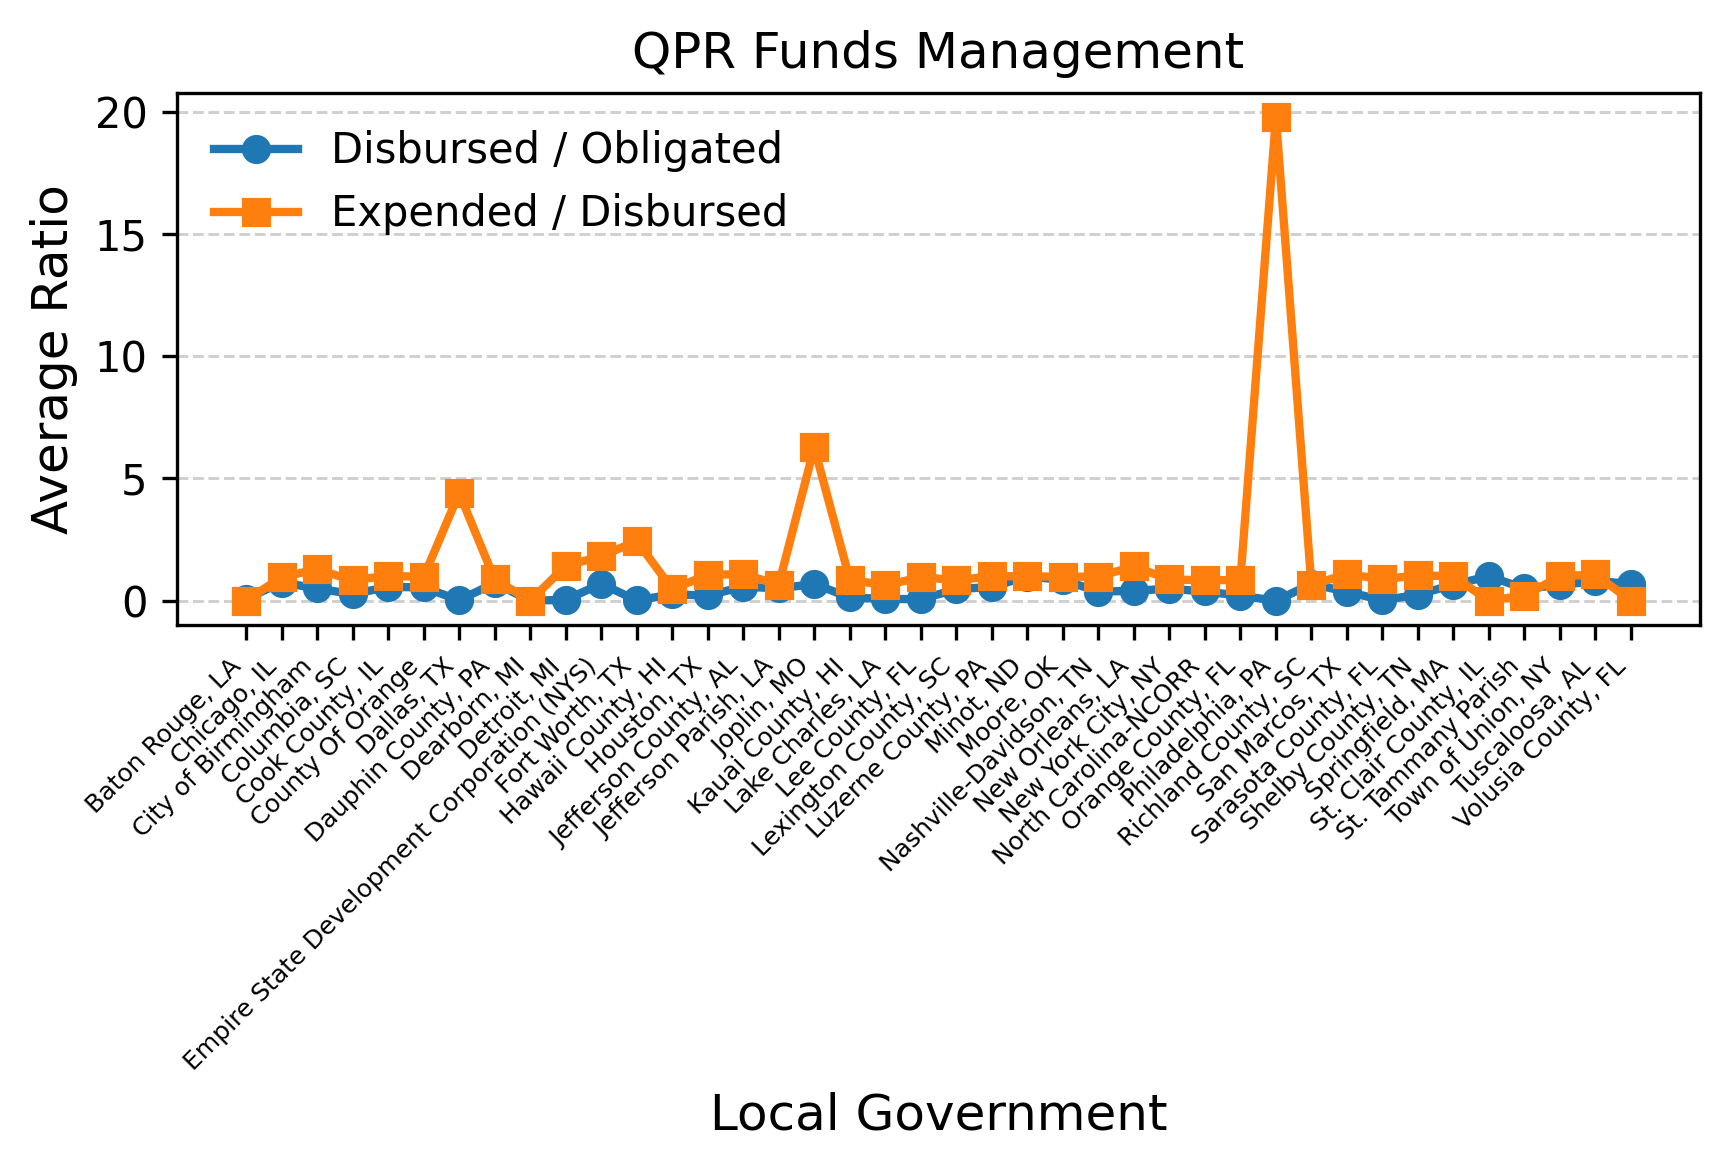
\includegraphics[keepaspectratio]{figures/fig_09_local_avg_ratios_2003_2023.png}}

}

\caption{Quarterly average local-level QPR ratios, again showing that
the main variation occurs before disbursement rather than after
disbursement.}

\end{figure}%

\subsection{Structural Estimates From Archived
Models}\label{structural-estimates-from-archived-models}

The structural results reinforce the exploratory reading. Table 2
reports selected coefficients from the archived diagnostics that matter
most for the audit.

\begin{longtable}[]{@{}
  >{\raggedright\arraybackslash}p{(\linewidth - 12\tabcolsep) * \real{0.1250}}
  >{\raggedright\arraybackslash}p{(\linewidth - 12\tabcolsep) * \real{0.1250}}
  >{\raggedright\arraybackslash}p{(\linewidth - 12\tabcolsep) * \real{0.1250}}
  >{\raggedleft\arraybackslash}p{(\linewidth - 12\tabcolsep) * \real{0.1667}}
  >{\raggedleft\arraybackslash}p{(\linewidth - 12\tabcolsep) * \real{0.1667}}
  >{\raggedleft\arraybackslash}p{(\linewidth - 12\tabcolsep) * \real{0.1667}}
  >{\raggedright\arraybackslash}p{(\linewidth - 12\tabcolsep) * \real{0.1250}}@{}}
\toprule\noalign{}
\begin{minipage}[b]{\linewidth}\raggedright
Specification
\end{minipage} & \begin{minipage}[b]{\linewidth}\raggedright
Analysis level
\end{minipage} & \begin{minipage}[b]{\linewidth}\raggedright
Subset
\end{minipage} & \begin{minipage}[b]{\linewidth}\raggedleft
N
\end{minipage} & \begin{minipage}[b]{\linewidth}\raggedleft
Throughput effect
\end{minipage} & \begin{minipage}[b]{\linewidth}\raggedleft
p-value
\end{minipage} & \begin{minipage}[b]{\linewidth}\raggedright
Interpretation
\end{minipage} \\
\midrule\noalign{}
\endhead
\bottomrule\noalign{}
\endlastfoot
Legacy \texttt{kaifa\_3x3\_full} & grantee & state & 36 & 113.652 &
\textless0.001 & Reproduces a large positive path, but only under
censored duration plus inverse-duration timeliness. \\
\texttt{exp\_optimal\_v1} & grantee & all & 40 & 0.320 & 0.958 &
Non-significant baseline. \\
\texttt{exp\_optimal\_v1} & grantee & state & 15 & 10.031 & 0.834 &
Non-significant and unstable. \\
\texttt{exp\_optimal\_v1} & grantee-disaster & state & 23 & 0.362 &
0.970 & Non-significant and unstable. \\
\texttt{exp\_time\_to\_milestone} & grantee-disaster & state & 52 &
-0.753 & 0.783 & Milestone timing alternative remains
non-significant. \\
\texttt{duration\_free\_cv} & grantee-disaster & all & 156 & 0.360 &
0.132 & Larger sample moves closer to zero-centered uncertainty, not to
a stable positive effect. \\
\end{longtable}

Two conclusions follow. First, the later Word manuscript's large
positive state coefficient cannot be treated as a general result of the
Kaifa framework. The archived replication can reproduce a large positive
path, but only in the specific legacy setup that combines right-censored
duration with its inverse on the throughput factor. Second, once the
indicator overlap is removed, the cross-sectional SEM does not produce a
robust or statistically convincing throughput-outcome relationship.

\subsection{State And Local Subsets Are Sensitivity Checks, Not
Moderation
Tests}\label{state-and-local-subsets-are-sensitivity-checks-not-moderation-tests}

The archive contains subset fit diagnostics for state and local
grantees, but the effective complete-case samples are 23 states and 17
local governments in the principal subset comparison. Those sample sizes
are too small to support formal claims that state and local governments
respond to throughput constraints in substantively different ways. This
is why the manuscript no longer uses the language of moderation. At
most, the subset results suggest that any state-versus-local comparison
is fragile and highly dependent on indicator choice. No formal
measurement invariance testing was conducted across government types,
and both subset samples fall well below conventional thresholds for
stable SEM estimation.

\section{Discussion}\label{discussion}

The core lesson from the audit is methodological rather than
substantive. The CDBG-DR QPR archive does contain useful information
about throughput variation, but it does not automatically yield a stable
cross-sectional SEM of latent administrative throughput. Three
constraints dominate.

First, the unit of analysis is difficult to justify. Aggregating
grantee-disaster histories to grantee means assumes that throughput is
stable enough across disaster events and policy periods to be summarized
as a single trait. That may be acceptable for exploratory screening, but
it is not a neutral choice. It removes temporal variation precisely
where a long-run administrative throughput story should be most
informative.

Second, the timing outcomes remain maturity-sensitive. Newer disasters
have had less time to reach any high completion threshold, and a 95
percent completion rule creates substantial right-censoring. The legacy
replication responds by treating incomplete programs as if they
completed at the current observation window, which mechanically biases
duration downward for ongoing programs. This is why the manuscript no
longer uses causal or deterministic language such as ``throughput
improves recovery outcomes'' or ``throughput shapes timeliness.'' The
archive supports only associational and design-diagnostic statements.
The positive association between the throughput summary and recovery
timeliness at the state level should therefore be characterized as a
pooled-descriptive result that is sensitive to maturity and cohort
composition. The sensitivity analyses in the archive show meaningful
attenuation rather than reassuring stability, which means the manuscript
cannot claim this as a robust structural relationship.

Third, the later Word draft extends beyond the reproducible archive.
QCEW staffing proxies, SVI covariates, and geography-matching logic may
be analytically valuable, but they need their own provenance rebuild. In
the current repository, those pieces cannot yet be documented with the
level of detail needed for publication-quality claims about suppression
handling, cross-vintage harmonization, or match-rate validation.

The practical implication is straightforward. If this manuscript is to
move beyond archival salvage, the next version should either:

\begin{enumerate}
\def\labelenumi{\arabic{enumi}.}
\tightlist
\item
  remain a narrow exploratory note centered on transparent model
  feasibility, or
\item
  be rebuilt around a longitudinal or survival-style design that
  respects event timing and censoring.
\end{enumerate}

The current redraft chooses the first path.

\section{Conclusion}\label{conclusion}

The Kaifa SEM archive remains useful, but not for the reason originally
claimed. It does not provide strong confirmatory evidence that a stable
latent administrative throughput construct explains cross-sectional
variation in CDBG-DR recovery outcomes. What it does provide is an
auditable record of why that conclusion is hard to sustain with the
available complete-case samples and indicator design.

For that reason, the present manuscript is best read as an exploratory
working paper and methodological archive. It documents descriptive
throughput differences across grantees, reconciles the archived model
comparison outputs, and shows that the strong positive legacy SEM result
is design-dependent. Future work can build on this record, but it should
do so with a redesigned temporal framework rather than by treating the
archived cross-sectional SEM as settled evidence.

\section{Data Availability Statement}\label{data-availability-statement}

The current reproducible manuscript archive relies primarily on public
HUD DRGR/QPR administrative data and project-generated derivative tables
stored in this repository. The archived robustness tables, Quarto source
files, and analysis code used for this redraft are available in the
repository. The April 7, 2026 Word draft also refers to external
covariates such as BLS QCEW and CDC/ATSDR SVI measures; those raw
sources are public, but the later joined linkage artifacts and
geography-validation files are not yet packaged as a reproducible
release in this archive. The current manuscript therefore distinguishes
between public raw sources, shareable code and nonrestricted
derivatives, and historical linkage artifacts that would need a separate
curation pass before distribution.

\section{References}\label{references}

Bollen, K. A. (1989). \emph{Structural Equations with Latent Variables}.
John Wiley \& Sons.

Boyd, E. (2011). \emph{Community Development Block Grant Disaster
Recovery Assistance}. Congressional Research Service.

Chang, S. E. (2010). Urban disaster recovery: A measurement framework
and its application to the 1995 Kobe earthquake. \emph{Disasters,
34}(2), 303-327.

Cutter, S. L., Ash, K. D., \& Emrich, C. T. (2019). Urban-rural
differences in disaster resilience. \emph{Annals of the American
Association of Geographers, 109}(5), 1237-1252.

Geddam, S. M., Garg, P., \& Tyagi, A. (2024). Enhancing disaster
management effectiveness: A structural equation modeling approach.
\emph{International Journal of Disaster Risk Reduction, 99}, 104123.

Gerber, B. J., \& Robinson, S. E. (2022). Local government capacity and
disaster resilience: The role of institutional arrangements and
administrative resources. \emph{Public Administration Review, 82}(2),
340-352.

HUD Office of Inspector General. (2021). \emph{HUD Did Not Adequately
Oversee Community Development Block Grant-Disaster Recovery Grantees}.
Office of Inspector General, U.S. Department of Housing and Urban
Development.

Kline, R. B. (2016). \emph{Principles and Practice of Structural
Equation Modeling} (4th ed.). Guilford Press.

Wu, X., Ramesh, M., \& Howlett, M. (2015). Policy capacity: A conceptual
framework for understanding policy competences and capabilities.
\emph{Policy and Society, 34}(3-4), 165-171.

\newpage

\section*{Appendix A: Data Description And
Provenance}\label{appendix-a-data-description-and-provenance}
\addcontentsline{toc}{section}{Appendix A: Data Description And
Provenance}

\subsection{A.1 Reproducible Source
Boundary}\label{a.1-reproducible-source-boundary}

The current Quarto archive is anchored to the reproducible project
pipeline rather than to the full set of variables discussed in the April
7, 2026 Word draft. The empirical results reported in this redraft come
from three repository artifacts:

\begin{enumerate}
\def\labelenumi{\arabic{enumi}.}
\tightlist
\item
  the standardized QPR archive
  (\texttt{data\_work/qpr\_standardized.parquet}),
\item
  the grantee-disaster feature panel
  (\texttt{data\_work/panel\_features.parquet}),
\item
  manuscript-specific robustness tables stored in
  \texttt{manuscript\_kaifa\_archive/data/} and
  \texttt{data\_work/diagnostics/}.
\end{enumerate}

The standardized QPR archive contains 130,605 activity-quarter rows.
Those rows are not one row per quarter; they are one row per activity
within a grantee-disaster-quarter. The cross-sectional SEM does not
estimate on that file directly. Instead, the canonical feature pipeline
collapses the QPR records to a grantee-disaster panel of 156
observations and then, for the Kaifa cross-sectional SEM, to one mean
profile per grantee.

\subsection{A.2 Transformation Chain}\label{a.2-transformation-chain}

The transformation chain relevant to the current manuscript is:

\begin{enumerate}
\def\labelenumi{\arabic{enumi}.}
\tightlist
\item
  QPR raw exports are cleaned and standardized into quarter-aware
  records.
\item
  Grantee-disaster features are computed, including financial ratios and
  timing summaries.
\item
  The archived Kaifa replication applies a legacy censoring rule:
  \texttt{Duration\_censored\ =\ N\_Quarters} whenever 95 percent
  completion is not observed.
\item
  The same legacy replication defines \texttt{Timeliness\_censored} as
  \texttt{1\ /\ Duration\_censored}.
\item
  The Kaifa cross-sectional SEM aggregates grantee-disaster measures to
  the grantee level using means.
\end{enumerate}

That chain matters because the positive legacy SEM result appears only
after steps 3 through 5. The current manuscript therefore treats those
steps as objects of audit, not as innocuous preprocessing choices.

\subsection{A.3 Sample Sizes Used In The
Archive}\label{a.3-sample-sizes-used-in-the-archive}

The main sample counts used in this redraft are:

\begin{longtable}[]{@{}
  >{\raggedright\arraybackslash}p{(\linewidth - 4\tabcolsep) * \real{0.3000}}
  >{\raggedleft\arraybackslash}p{(\linewidth - 4\tabcolsep) * \real{0.4000}}
  >{\raggedright\arraybackslash}p{(\linewidth - 4\tabcolsep) * \real{0.3000}}@{}}
\toprule\noalign{}
\begin{minipage}[b]{\linewidth}\raggedright
Sample
\end{minipage} & \begin{minipage}[b]{\linewidth}\raggedleft
N
\end{minipage} & \begin{minipage}[b]{\linewidth}\raggedright
Notes
\end{minipage} \\
\midrule\noalign{}
\endhead
\bottomrule\noalign{}
\endlastfoot
Grantee-disaster feature panel & 156 & All grantee-disaster pairs in the
working panel. \\
Unique grantees & 78 & Cross-sectional aggregation target. \\
Disaster types & 18 & Disaster contexts represented in the panel. \\
\texttt{full} and \texttt{reduced} SEM complete cases & 41 & Overall
cross-sectional SEM sample in the manuscript archive. \\
\texttt{exp\_optimal\_v1} and related non-circular SEMs & 40 & Overall
baseline cross-sectional SEM sample. \\
State subset fit comparison & 23 & Complete cases in archived
subset-comparison table. \\
Local subset fit comparison & 17 & Complete cases in archived
subset-comparison table. \\
Legacy Kaifa state replication & 36 & Grantee-level state sample after
right-censoring and aggregation. \\
\end{longtable}

These counts should be read as complete-case estimation samples, not as
the total amount of information in the QPR archive.

\subsection{A.4 Timing And Maturity
Limits}\label{a.4-timing-and-maturity-limits}

The current redraft refers to disaster cohorts from 2003 through 2023.
Internally, the standardized QPR archive contains quarterly observations
from September 30, 2002 through June 30, 2025. The absolute dates matter
because the 95 percent completion rule is maturity-sensitive. More
recent disasters have had fewer reporting quarters in which to approach
the completion threshold, which is why duration-based outcomes are
vulnerable to right-censoring and cohort bias.

The archive also documents a minimum-quarter filter and ratio
winsorization. The historical Kaifa workflow excluded very short
reporting histories and used ratio trimming or winsorization to reduce
extreme values. The current redraft reports only those preprocessing
rules that can be traced in the repository and does not claim an
additional outlier-deletion procedure that cannot be reconstructed
cleanly.

\subsection{A.5 External Data Referenced In The Later Word
Draft}\label{a.5-external-data-referenced-in-the-later-word-draft}

The April 7, 2026 Word manuscript references additional external
sources, including:

\begin{itemize}
\tightlist
\item
  BLS QCEW staffing and payroll measures, including NAICS
  \texttt{925110},
\item
  CDC/ATSDR Social Vulnerability Index (SVI) vintages,
\item
  organization-name cleaning and city-to-county geography matching.
\end{itemize}

Those inputs were not initially reconstructed in the repository. A later
manual import added two external SEM export bundles under
\texttt{manuscript\_kaifa\_archive/data/external\_sem\_exports/}:

\begin{itemize}
\tightlist
\item
  \texttt{baseline\_sem/} with a 573-row z-scored ready dataset and
  associated one-factor/two-factor SEM exports;
\item
  \texttt{baseline\_sem\_admin\_4/} with a 169-row robustness version of
  the same variable family.
\end{itemize}

These imports are useful for provenance and for reconstructing the later
Word manuscript's SEM tables, but they still do not by themselves
document the upstream QCEW acquisition, SVI harmonization, or
geography-matching workflow. If those variables are reintroduced as
active empirical inputs, the following documentation is still required:

\begin{itemize}
\tightlist
\item
  for QCEW: extraction year coverage, suppression or missingness
  handling, and a clear statement that NAICS \texttt{925110} is an
  indirect proxy for CDBG-DR administrative capacity rather than a
  direct staff count;
\item
  for SVI: either a harmonization protocol across vintages or a design
  that avoids direct comparison of percentile scores across incompatible
  releases;
\item
  for geography matching: a source hierarchy, match shares by method,
  unresolved cases, and validation against official Census relationship
  or gazetteer files.
\end{itemize}

\subsection{A.6 Public, Shareable, And Controlled
Artifacts}\label{a.6-public-shareable-and-controlled-artifacts}

For the current manuscript archive, the data-availability boundary is:

\begin{itemize}
\tightlist
\item
  public raw sources: HUD DRGR/QPR administrative exports used in the
  repository, plus public federal data sources that may be used in
  future extensions such as Census population series, BLS QCEW, and
  CDC/ATSDR SVI;
\item
  shareable derivative materials: the Quarto manuscript sources, the
  repository code, and the archived robustness or audit tables used in
  this redraft;
\item
  controlled or not-yet-packaged materials: any historical manual
  linkage tables, reviewed geography crosswalks, or joined external-data
  artifacts referenced only in the later Word draft.
\end{itemize}

\newpage

\section*{Appendix B: Methodological
Details}\label{appendix-b-methodological-details}
\addcontentsline{toc}{section}{Appendix B: Methodological Details}

\subsection{B.1 SEM Families Compared In The
Archive}\label{b.1-sem-families-compared-in-the-archive}

The current Quarto archive compares three classes of SEM specification.
In all cases, the measurement model is treated as an exploratory latent
summary rather than a confirmed reflective structure. The indicators may
function as formative components (determinants of throughput) rather
than reflective manifestations (effects of a latent trait), and the
specifications adopted here do not distinguish between these
alternatives.

\begin{enumerate}
\def\labelenumi{\arabic{enumi}.}
\tightlist
\item
  \texttt{full} legacy models, which use censored duration and
  inverse-duration timeliness.
\item
  non-circular baseline models such as \texttt{exp\_optimal\_v1}, which
  remove the deterministic overlap between capacity and outcome timing.
\item
  alternative indicator models, such as milestone and duration-free
  variants, used only for sensitivity checks.
\end{enumerate}

No moderation model is estimated in the reproducible archive. State
versus local results are subset comparisons, not interaction tests,
multi-group invariance analyses, or moderation estimates.

\subsection{B.2 Legacy Replication Versus Preferred
Baseline}\label{b.2-legacy-replication-versus-preferred-baseline}

The legacy Kaifa replication is:

\[
\text{gov\_cap} =~ \text{Ratio\_disbursed\_to\_obligated} + \text{Ratio\_expended\_to\_disbursed} + \text{Timeliness\_censored}
\]

\[
\text{recovery\_outcome} =~ \text{Duration\_censored} + \text{Ratio\_obligated\_funds\_fully\_expended} + \text{Quarter\_by\_quarter\_variance\_expended}
\]

\[
\text{recovery\_outcome} \sim \text{gov\_cap}
\]

The preferred baseline for this redraft is the simpler non-circular
model:

\[
\text{gov\_cap} =~ \text{Ratio\_disbursed\_to\_obligated} + \text{Ratio\_expended\_to\_disbursed}
\]

\[
\text{recovery\_outcome} =~ \text{Duration\_log} + \text{Spending\_CV}
\]

\[
\text{recovery\_outcome} \sim \text{gov\_cap}
\]

The baseline is not presented as a well-validated measurement model. It
is simply the least problematic archived specification because it avoids
the timeliness-duration circularity.

\subsection{B.3 Why The Legacy Timing Construction Is
Problematic}\label{b.3-why-the-legacy-timing-construction-is-problematic}

The legacy manuscript replication defines:

\[
\text{Duration\_censored}_i =
\begin{cases}
\text{Duration}_i, & \text{if 95\% completion is observed} \\
\text{N\_Quarters}_i, & \text{otherwise}
\end{cases}
\]

and then

\[
\text{Timeliness\_censored}_i = \frac{1}{\text{Duration\_censored}_i}
\]

This means a single underlying duration quantity enters the SEM twice:
once directly on the outcome factor and once inversely on the capacity
factor. That is why the legacy positive path cannot be treated as clean
evidence for an underlying capacity effect.

\subsection{B.4 Measurement Evidence Available In The
Archive}\label{b.4-measurement-evidence-available-in-the-archive}

The archive contains parameter tables for selected specifications, but
it does not contain a complete package of residual matrices, construct
reliability statistics, or standardized latent-correlation tables for
every model in the later Word draft. The current manuscript therefore
reports the available evidence transparently and states what is missing.

\subsubsection{\texorpdfstring{Baseline \texttt{exp\_optimal\_v1}
Loadings And Structural Path (All
Grantees)}{Baseline exp\_optimal\_v1 Loadings And Structural Path (All Grantees)}}\label{baseline-exp_optimal_v1-loadings-and-structural-path-all-grantees}

\begin{longtable}[]{@{}lrrr@{}}
\toprule\noalign{}
Parameter & Estimate & Standard error & p-value \\
\midrule\noalign{}
\endhead
\bottomrule\noalign{}
\endlastfoot
\texttt{recovery\_outcome\ \textasciitilde{}\ gov\_cap} & 0.320 & 6.137
& 0.958 \\
\texttt{Ratio\_expended\_to\_disbursed\ \textasciitilde{}\ gov\_cap} &
-0.102 & 1.977 & 0.959 \\
\texttt{Spending\_CV\ \textasciitilde{}\ recovery\_outcome} & -0.367 &
2.174 & 0.866 \\
\end{longtable}

\subsubsection{\texorpdfstring{Legacy \texttt{kaifa\_3x3\_full} State
Replication}{Legacy kaifa\_3x3\_full State Replication}}\label{legacy-kaifa_3x3_full-state-replication}

\begin{longtable}[]{@{}
  >{\raggedright\arraybackslash}p{(\linewidth - 6\tabcolsep) * \real{0.2000}}
  >{\raggedleft\arraybackslash}p{(\linewidth - 6\tabcolsep) * \real{0.2667}}
  >{\raggedleft\arraybackslash}p{(\linewidth - 6\tabcolsep) * \real{0.2667}}
  >{\raggedleft\arraybackslash}p{(\linewidth - 6\tabcolsep) * \real{0.2667}}@{}}
\toprule\noalign{}
\begin{minipage}[b]{\linewidth}\raggedright
Parameter
\end{minipage} & \begin{minipage}[b]{\linewidth}\raggedleft
Estimate
\end{minipage} & \begin{minipage}[b]{\linewidth}\raggedleft
Standard error
\end{minipage} & \begin{minipage}[b]{\linewidth}\raggedleft
p-value
\end{minipage} \\
\midrule\noalign{}
\endhead
\bottomrule\noalign{}
\endlastfoot
\texttt{recovery\_outcome\ \textasciitilde{}\ gov\_cap} & 113.652 &
17.535 & \textless0.001 \\
\texttt{Ratio\_expended\_to\_disbursed\ \textasciitilde{}\ gov\_cap} &
1.254 & 1.305 & 0.337 \\
\texttt{Timeliness\_censored\ \textasciitilde{}\ gov\_cap} & -0.273 &
0.075 & \textless0.001 \\
\texttt{Ratio\_obligated\_funds\_fully\_expended\ \textasciitilde{}\ recovery\_outcome}
& 0.0106 & 0.0011 & \textless0.001 \\
\texttt{Quarter\_by\_quarter\_variance\_expended\ \textasciitilde{}\ recovery\_outcome}
& -0.0001 & 0.0006 & 0.831 \\
\end{longtable}

These tables are enough to show why the legacy result looks strong and
why the baseline result does not. They are not enough to claim full
construct validation. The missing elements are therefore treated as a
methodological limitation, not as information that can be inferred away.

A rigorous measurement validation would require confirmatory factor
analysis on a hold-out sample with adequate power (conventionally N
\textgreater{} 200 per group), comparison of reflective versus formative
specifications using MIMIC or PLS-SEM, and convergent and discriminant
validity testing against external indicators such as staffing levels or
prior program experience. None of these steps were feasible given the
available complete-case samples (N = 40 overall, N = 23 state, N = 17
local).

\subsection{B.5 Fit Interpretation}\label{b.5-fit-interpretation}

Fit indices are reported exactly as archived, but they are interpreted
with two cautions.

\begin{enumerate}
\def\labelenumi{\arabic{enumi}.}
\tightlist
\item
  Very small SEM samples with low degrees of freedom can produce
  unstable or non-intuitive fit values, including CFI or TLI estimates
  above 1.
\item
  No model in the current archive satisfies a clean combination of
  strong incremental fit, acceptable absolute fit, and conceptually
  non-overlapping indicators.
\end{enumerate}

For that reason, the redraft does not declare a single preferred
confirmatory measurement model. It instead uses the comparison table to
document the tradeoffs across archived specifications.

\subsection{B.6 Metrics Excluded From The Current
Redraft}\label{b.6-metrics-excluded-from-the-current-redraft}

The later Word draft introduced administrative gap measures and a
Recovery Governance Risk Index. Those metrics are not interpreted in the
current Quarto redraft because the repository does not contain a fully
reproducible set of equations, weights, and sensitivity tables for that
extension. The review concern is handled by removing unsupported metric
claims from the current manuscript rather than by reverse-engineering
unverified formulas.

\subsection{B.7 Interpretation Rule}\label{b.7-interpretation-rule}

All throughput-outcome relationships in this manuscript are interpreted
as associational and exploratory. The manuscript does not claim
moderation, causal identification, or stable state-versus-local effect
heterogeneity.

\newpage

\section*{Appendix C: Robustness And Audit
Tables}\label{appendix-c-robustness-and-audit-tables}
\addcontentsline{toc}{section}{Appendix C: Robustness And Audit Tables}

\subsection{C.1 Archived Specification
Comparison}\label{c.1-archived-specification-comparison}

\begin{longtable}[]{@{}
  >{\raggedright\arraybackslash}p{(\linewidth - 16\tabcolsep) * \real{0.0857}}
  >{\raggedleft\arraybackslash}p{(\linewidth - 16\tabcolsep) * \real{0.1143}}
  >{\raggedleft\arraybackslash}p{(\linewidth - 16\tabcolsep) * \real{0.1143}}
  >{\raggedleft\arraybackslash}p{(\linewidth - 16\tabcolsep) * \real{0.1143}}
  >{\raggedleft\arraybackslash}p{(\linewidth - 16\tabcolsep) * \real{0.1143}}
  >{\raggedleft\arraybackslash}p{(\linewidth - 16\tabcolsep) * \real{0.1143}}
  >{\raggedleft\arraybackslash}p{(\linewidth - 16\tabcolsep) * \real{0.1143}}
  >{\raggedleft\arraybackslash}p{(\linewidth - 16\tabcolsep) * \real{0.1143}}
  >{\raggedleft\arraybackslash}p{(\linewidth - 16\tabcolsep) * \real{0.1143}}@{}}
\toprule\noalign{}
\begin{minipage}[b]{\linewidth}\raggedright
Model
\end{minipage} & \begin{minipage}[b]{\linewidth}\raggedleft
chi2
\end{minipage} & \begin{minipage}[b]{\linewidth}\raggedleft
chi2 p-value
\end{minipage} & \begin{minipage}[b]{\linewidth}\raggedleft
CFI
\end{minipage} & \begin{minipage}[b]{\linewidth}\raggedleft
TLI
\end{minipage} & \begin{minipage}[b]{\linewidth}\raggedleft
RMSEA
\end{minipage} & \begin{minipage}[b]{\linewidth}\raggedleft
AIC
\end{minipage} & \begin{minipage}[b]{\linewidth}\raggedleft
BIC
\end{minipage} & \begin{minipage}[b]{\linewidth}\raggedleft
N
\end{minipage} \\
\midrule\noalign{}
\endhead
\bottomrule\noalign{}
\endlastfoot
\texttt{full} & 15.384 & 0.052 & 0.938 & 0.883 & 0.152 & 25.250 & 47.526
& 41 \\
\texttt{reduced} & 56.315 & \textless0.001 & 0.498 & -0.256 & 0.572 &
19.253 & 38.102 & 41 \\
\texttt{exp\_optimal\_v1} & 0.022 & 0.882 & 0.790 & -0.259 & 0.000 &
17.999 & 33.199 & 40 \\
\texttt{exp\_optimal\_v2} & 2.710 & 0.608 & 0.758 & 0.394 & 0.000 &
21.865 & 40.442 & 40 \\
\texttt{improved\_3x3} & 4.094 & 0.848 & 1.486 & 1.911 & 0.000 & 25.795
& 47.751 & 40 \\
\texttt{improved\_3x3\_progress} & 57.005 & \textless0.001 & 0.238 &
-0.430 & 0.396 & 23.150 & 45.105 & 40 \\
\end{longtable}

\subsection{C.2 Archived Subset
Comparison}\label{c.2-archived-subset-comparison}

\begin{longtable}[]{@{}
  >{\raggedright\arraybackslash}p{(\linewidth - 16\tabcolsep) * \real{0.0857}}
  >{\raggedleft\arraybackslash}p{(\linewidth - 16\tabcolsep) * \real{0.1143}}
  >{\raggedleft\arraybackslash}p{(\linewidth - 16\tabcolsep) * \real{0.1143}}
  >{\raggedleft\arraybackslash}p{(\linewidth - 16\tabcolsep) * \real{0.1143}}
  >{\raggedleft\arraybackslash}p{(\linewidth - 16\tabcolsep) * \real{0.1143}}
  >{\raggedleft\arraybackslash}p{(\linewidth - 16\tabcolsep) * \real{0.1143}}
  >{\raggedleft\arraybackslash}p{(\linewidth - 16\tabcolsep) * \real{0.1143}}
  >{\raggedleft\arraybackslash}p{(\linewidth - 16\tabcolsep) * \real{0.1143}}
  >{\raggedleft\arraybackslash}p{(\linewidth - 16\tabcolsep) * \real{0.1143}}@{}}
\toprule\noalign{}
\begin{minipage}[b]{\linewidth}\raggedright
Subset
\end{minipage} & \begin{minipage}[b]{\linewidth}\raggedleft
chi2
\end{minipage} & \begin{minipage}[b]{\linewidth}\raggedleft
chi2 p-value
\end{minipage} & \begin{minipage}[b]{\linewidth}\raggedleft
CFI
\end{minipage} & \begin{minipage}[b]{\linewidth}\raggedleft
TLI
\end{minipage} & \begin{minipage}[b]{\linewidth}\raggedleft
RMSEA
\end{minipage} & \begin{minipage}[b]{\linewidth}\raggedleft
AIC
\end{minipage} & \begin{minipage}[b]{\linewidth}\raggedleft
BIC
\end{minipage} & \begin{minipage}[b]{\linewidth}\raggedleft
N
\end{minipage} \\
\midrule\noalign{}
\endhead
\bottomrule\noalign{}
\endlastfoot
all grantees & 0.022 & 0.882 & 0.790 & -0.259 & 0.000 & 17.999 & 33.199
& 40 \\
state grantees & 2.134 & 0.144 & 1.379 & 3.276 & 0.227 & 17.814 & 28.034
& 23 \\
local grantees & 2.209 & 0.137 & 1.372 & 3.233 & 0.275 & 17.740 & 25.239
& 17 \\
\end{longtable}

The subset table is retained only as a sensitivity check. The fit values
are too unstable for strong inference, and the sample sizes are too
small to support a formal state-versus-local comparison.

\subsection{C.3 Alternative Outcome
Specifications}\label{c.3-alternative-outcome-specifications}

\begin{longtable}[]{@{}
  >{\raggedright\arraybackslash}p{(\linewidth - 12\tabcolsep) * \real{0.1154}}
  >{\raggedright\arraybackslash}p{(\linewidth - 12\tabcolsep) * \real{0.1154}}
  >{\raggedleft\arraybackslash}p{(\linewidth - 12\tabcolsep) * \real{0.1538}}
  >{\raggedleft\arraybackslash}p{(\linewidth - 12\tabcolsep) * \real{0.1538}}
  >{\raggedleft\arraybackslash}p{(\linewidth - 12\tabcolsep) * \real{0.1538}}
  >{\raggedleft\arraybackslash}p{(\linewidth - 12\tabcolsep) * \real{0.1538}}
  >{\raggedleft\arraybackslash}p{(\linewidth - 12\tabcolsep) * \real{0.1538}}@{}}
\toprule\noalign{}
\begin{minipage}[b]{\linewidth}\raggedright
Model
\end{minipage} & \begin{minipage}[b]{\linewidth}\raggedright
Subset
\end{minipage} & \begin{minipage}[b]{\linewidth}\raggedleft
N
\end{minipage} & \begin{minipage}[b]{\linewidth}\raggedleft
CFI
\end{minipage} & \begin{minipage}[b]{\linewidth}\raggedleft
RMSEA
\end{minipage} & \begin{minipage}[b]{\linewidth}\raggedleft
Throughput beta
\end{minipage} & \begin{minipage}[b]{\linewidth}\raggedleft
p-value
\end{minipage} \\
\midrule\noalign{}
\endhead
\bottomrule\noalign{}
\endlastfoot
\texttt{duration\_free\_cv} & all & 156 & 0.990 & 0.105 & 0.360 &
0.132 \\
\texttt{duration\_free\_cv} & state & 94 & 0.979 & 0.163 & 0.326 &
0.179 \\
\texttt{duration\_free\_cv} & local & 61 & 0.968 & 0.164 & 0.337 &
0.431 \\
\texttt{milestone\_time\_to\_50} & all & 156 & 0.758 & 0.308 & -0.365 &
0.354 \\
\texttt{milestone\_time\_to\_50} & state & 94 & 0.983 & 0.093 & -0.442 &
0.404 \\
\texttt{milestone\_time\_to\_50} & local & 61 & 0.691 & 0.434 & -0.266 &
0.617 \\
\texttt{milestone\_progress\_rate} & all & 156 & 0.847 & 0.092 & 0.091 &
0.685 \\
\texttt{milestone\_velocity} & all & 156 & 0.995 & 0.209 & 0.014 &
0.669 \\
\end{longtable}

Across the alternative designs, the non-circular SEMs remain
non-significant. Expanding the sample through duration-free or
milestone-based outcomes does not recover a stable positive throughput
effect.

\subsection{C.4 Outlier And Preprocessing
Note}\label{c.4-outlier-and-preprocessing-note}

The current archive documents winsorization or trimming of extreme ratio
values in preprocessing, but it does not contain a manuscript-specific
table that cleanly reconstructs an additional outlier-removal robustness
pass from the later Word draft. For transparency, the redraft does not
claim a separate outlier-deletion result. The reader should treat the
archived robustness evidence as limited to the specification, subset,
and alternative outcome tables reported here.

\subsection{C.5 Robustness Conclusion}\label{c.5-robustness-conclusion}

The robustness archive points in one direction. The large positive SEM
path appears only in the legacy censored-duration replication. Once the
timing overlap is removed or the outcome is redefined, the structural
path is no longer statistically persuasive.




\end{document}
